% \documentclass[12pt,draftclsnofoot,peerreview,onecolumn]{IEEEtran}
\documentclass[journal,comsoc]{IEEEtran}
\usepackage[T1]{fontenc}
% \usepackage{cite}
% \usepackage{amsfonts}
\usepackage{amssymb}
\usepackage{amsmath}
\interdisplaylinepenalty=2500
\usepackage{filecontents}
\usepackage{url}
\usepackage{bm}
\usepackage[square,sort,comma,numbers]{natbib}
\usepackage{subfigure} 
% \usepackage{caption}
% \usepackage{subcaption}
\usepackage[colorlinks,
  linkcolor=black,
  anchorcolor=blue,
  citecolor=black
  ]{hyperref}
\ifCLASSINFOpdf
 \usepackage[pdftex]{graphicx}
\else
 \usepackage[dvips]{graphicx}
\fi

% correct bad hyphenation here
\hyphenation{op-tical net-works semi-conduc-tor}

\renewcommand{\citedash}{--}

\DeclareMathOperator*{\argmax}{arg\,max}

\begin{document}
%
% paper title
% can use linebreaks \\ within to get better formatting as desired

\title{Entropy Minimization Based Symbol Timing
\\and Carrier Frequency Recovery}
% \author{\IEEEauthorblockN{Xiao Liu and Jean-Fran\c{c}ois Bousquet }
% \IEEEauthorblockA{Electrical and Computer Engineering\\
% Dalhousie University\\
% Halifax, B3H 4R2, Canada\\
% Email: x.liu@dal.ca}}
\author{Xiao~Liu,~\IEEEmembership{Student Member,~IEEE,}
%         John~Doe,~\IEEEmembership{Fellow,~OSA,}
        and~Jean-Fran\c{c}ois~Bousquet,~\IEEEmembership{Member,~IEEE}% <-this % stops a space

\thanks{Manuscript received April 8, 2017; revised xxxx xx, 2017. This project was supported by the Atlantic Innovation Fund \#Project \#203162.}
\thanks{The authors are with the Department of Electrical and Computer Engineering, Dalhousie University, Halifax,
NS, B3J 1Z1, Canada (e-mail: \{x.liu, jbousquet\}@dal.ca).}% <-this % stops a space
% \thanks{J. Bousquet is with Dalhousie University.}% <-this % stops a space
}

% The paper headers
\markboth{IEEE Transactions on Wireless Communications,~Vol.~xx, No.~x, xxxxxx~2017}%
{Shell \MakeLowercase{\textit{et al.}}: Entropy Minimization Based Symbol Timing and Carrier Frequency Recovery}

% make the title area
\maketitle


\begin{abstract}
This paper  presents a new entropy minimization criterion that is used for both symbol timing and carrier frequency recovery in a wireless receiver.
It relies on the entropy estimation of the eye diagram and the constellation diagram of the received signal. 
During the parameter search, when the perfect synchronization is achieved, the entropy will reach a sharp global minimum, indicating the least intersymbol interference or a restored constellation diagram. 
% The minimized entropy indicates a regular pattern with the least interference, that is where the signal is synchronized and recovered correctly.
% In the synchronization parameter search, the corresponding entropy reaches a sharp global minimum when the signal is recovered correctly.
Unlike other synchronization methods, this unified criterion can be used to build an all-in-one synchronizer with high accuracy.
The feasibility of this method is proven using a theoretical analysis and supported with numerical simulation. 
\end{abstract}

% {\bf Keywords:} 
\begin{IEEEkeywords}
Entropy minimization, symbol timing, carrier frequency recovery, synchronization.
\end{IEEEkeywords}

\IEEEpeerreviewmaketitle

\section{Introduction}
\label{sec:intro}
\IEEEPARstart{S}{ynchronization} is essential in wireless coherent receivers.
It is usually realized between the matched filter and the equalizer.
The two main functions of the synchronizer are symbol timing and carrier recovery.
The purpose of symbol timing recovery is to recover the symbol clock from the modulated waveform, so that it can sample the waveform at the correct \textit{symbol rate} and \textit{timing phase}.
With proper pulse shaping, matched filter and symbol timing, the data samples will have maximum signal to noise ratio (SNR) and no intersymbol interference (ISI)~\cite{mengali1997synchronization}.
Also, coherent demodulation of a passband signal requires exactly the same carrier frequency and phase. 
The receiver usually has an independent local oscillator to generate the carrier reference which deviates from the signal.  
Thus, the synchronizer has to compensate for the carrier frequency offset (CFO). 
In some applications, such as underwater acoustic communication, the channel may constantly change due to the time-variant channel or Doppler effect. 
Therefore a continuous estimation and compensation of the synchronization error is essential to maintain the link reliability.

% \textbf{a summary of standard solutions }
Various synchronization schemes have been proposed in the literature.
They are generally characterized by their structures and the availability of training data.
The \textit{feedforward} structure directly extracts the timing tone or CFO  from the incoming signal.
Whereas the \textit{feedback} structure uses a timing (or frequency) error detector to derive an error signal and feeds it back to recover the synchronization parameters.
On the other hand, if the training data is available, we say the algorithm is \textit{supervised}, otherwise it is \textit{unsupervised}.
This categorization is also known as \textit{data-aided} (DA), \textit{decision-directed} (DD) and \textit{non-data-aided} (NDA) \cite{mengali1997synchronization}.

Except for few ad-hoc algorithms, all these synchronization schemes follow maximum likelihood (ML) criterion or its approximation.
For example, the O\&M algorithm \cite{Oerder1988}, a magnitude-squared nonlinear spectral line method exploiting the cyclostationary properties of the modulated signal, is one of the most commonly used unsupervised  feedforward scheme for symbol timing recovery.
It has been proved that this algorithm and its modifications can be asymptotically interpreted as ML estimators \cite{YanWang2002,Lopez-Salcedo2006}.
Regarding the carrier recovery, the algorithms derived from ML criterion are trying to maximize the inner product between the  training sequence and the data samples (DA, DD) or the energy of the matched filter output (NDA) \cite{mengali1997synchronization}.

% \textbf{What is scope of this paper }
In this paper, we consider an alternative criterion that minimizes the entropy of the data samples. 
Like the ML criterion, it aims to optimize a unified objective function.
The scheme we will focus on is unsupervised and implemented in a feedforward receiver structure, but can be extended to other configurations in the future under the same criterion.
Note that it has been shown in~\cite{Pedzisz2006} that the carrier frequency offset of the phase-shift keying (PSK) signals can be recovered by minimizing the entropy of the instantaneous phase probability density function.
% Also, it has been reported that the error entropy minimization algorithms can be applied for channel equalization \cite{Santamaria2002}. 
However, to the authors' knowledge,  the unified criterion for both symbol timing and carrier recovery with linear modulation schemes has not been studied.

Since Shannon's work, entropy~\cite{Shannon1948} is used as a major tool in information theory. 
But except for theoretical analysis, it is rarely used in signal processing because of its complexity~\cite{Bercher2000}.
Exceptionally, in the study of physiological data, researchers use simplified approximate entropy (ApEn)~\cite{Pincus1991}, or sample entropy (SampEn)~\cite{Richman2000} to estimate the complexity of the time series.
Likewise, we will propose an ad-hoc entropy estimation algorithm to accelerate the synchronization searching. 

% PMF not PDF
% Unlike these systems, this paper focuses on
%  \textbf{contributions}
The contribution of this work is summarized as below.
1)~The entropy minimization (EM) criterion is studied for symbol timing and carrier frequency recovery.
2)~An ad-hoc entropy estimation algorithm is proposed for fast parameter estimation.
3)~The practical issues of EM based synchronization algorithms is discussed. 

\textbf{organization...}

Preliminary results on this subject presented in [13] are here extended and consolidated in terms of
This paper is organized as follows.

In Section II,

In Section III,

performance analysis with simulation and sea trial data is investigated in Section \ref{sec:performance}. 
Finally, conclusions are drawn in Section \ref{sec:conc}.
% \clearpage
%%%%%%%%%%%%%%%%%%%%%%%%%%%%%%%%%%%%%%%%%%%%%%%%%%

\section{Entropy as a Cost Function for Synchronization}
\label{sec:entropy}
In this section, the signal model and the basics of Shannon information entropy are briefly introduced.
% we are going to use through this article.
Then, the EM criterion is applied to symbol timing and carrier frequency recovery with the help of eye diagram and constellation diagram.
% An ad-hoc entropy estimation algorithm is proposed in the last part of this section for fast synchronization parameter search.
\subsection{Signal model }  

% There are other forms of definitions or expressions of entropy that won't be detailed here.
% We will focus on how entropy can be applied in symbol timing and carrier frequency recovery.

In this work, it is assumed that the signal is linearly modulated, such as PSK or QAM (quadrature amplitude modulation), etc., with an alphabet size of \(M\), where \(M\) is usually a power of 2.
The bit stream follows an independent identical distribution.
The modulated data is pulse shaped through a pulse shaping filter to limit the bandwidth occupancy.
The root-raised-cosine (RRC) filter is chosen as the pulse shaping filter, which is designed under the Nyquist criterion, 
such that there is no ISI at the proper sampling instants.
\begin{figure*}[ht]
\centering
\includegraphics[width=5.5 in]{pic/sys_conf.png}
\caption{Block diagram of the receiver configuration.}
\label{fig:sysconf} 
\end{figure*}

Fig. \ref{fig:sysconf} shows the block diagram of the receiver configuration.
The down conversion is done first, but the CFO may still exist after it.
The matched filter is the same RRC filter used in pulse shaping , so the over all filter becomes a raised-cosine (RC) filter. 
Then the timing recovery is applied prior to carrier recovery.
Provided timing is known, the decimated samples (usually one or two samples per symbol) are sufficient for CFO recovery.
Also, if the symbol timing is recovered first, the carrier recovery will have less computational burden due to the decimation of samples.
Therefore, the preferred sequence in this work is to apply symbol timing before carrier frequency recovery, but it is not rigid.

The data samples \(x_i\) after timing and carrier frequency recovery can be expressed as
\begin{equation}
{x_i}( \tau ,{f_\Delta }) = y(iT +  \tau ){e^{ - j2\pi {f_\Delta }iT}},
\end{equation}
where \(y\) is the output of the matched filter, \(\tau\) and \(f_\Delta\) are the timing phase and the CFO respectively.


\subsection{Maximum Likelihood Versus Entropy Minimization}
Conventional synchronization methods intend to maximize the likelihood functions.
For instance, in the NDA timing phase estimation, this criterion yields an objective function
\begin{equation}
\Lambda(\tau) =\sum\limits_{i = 1}^N {{{\left| {{x_i}( \tau )} \right|}^2}}, 
\end{equation}
while the DA carrier frequency recovery often uses an objective function equal to
\begin{equation}
\Lambda ({\Delta f_c })=\sum\limits_{i = 1}^N {{{\left| {c_i^*{x_i}(\tau ,{f_\Delta })} \right|}}}. 
\end{equation}
where \(c_i^*\) is the complex conjugate of the \(i\)-th training data.
If we take a close look at these two likelihood functions, they are actually aimed at achieving the the same objective, which is to maximize the energy of the data samples.
This type of estimation method uses second-order statistics and is suitable for linear channels with Gaussian noise.
Without the linearity and Gaussianity assumption, a criterion considering the higher order statistics would be appropriate.
The entropy is a measure of randomness or uncertainty of this signal, and it is a function of the signal probability density function (PDF).
By using entropy instead of likelihood function, the higher order statistics are taken into consideration \cite{Santamaria2002}.

The Shannon entropy is a measure of the quantity of information  embedded in a signal.
% In fact, we can also consider it as a measure of randomness or uncertainty of this signal.
% The most common approach to estimate the entropy is defined below.
% This Shannon entropy of discrete signal is defined below.
Assuming \(k\) possible observations of a one-dimensional discrete signal, with \(p_i\) representing the probability of the \(i\)-th possibility, the information entropy \(H_S\) is commonly expressed as \cite{Shannon1948}
\begin{equation}
H_S =  - \sum\limits_{i = 1}^k {{p_i}\log {p_i}}.
\label{eq:entropy}
\end{equation}
The base of the logarithmic function is usually chosen to be 2, and the corresponding entropy unit is \textit{bits}.
Next, we will use entropy as a metric to evaluate the eye diagram and constellation diagram.

\subsection{Eye Diagram and Timing Phase Entropy}
\label{sec:eye_entp}
To recover the symbol timing, the entropy of the eye diagram is utilized. 
% The eye diagram is a graphical illustration that consists of many periodically overlaid traces of short windows of a signal.
% Normally, the length of the segment is one or two symbol periods. 
The symbol timing recovery problem can be then interpreted as estimating the adequate timing phase on the eye diagram.
The ideal down-sampling instant is located in the middle of the eye diagram where the eye opening reaches its maximum.
% Fig. \ref{fig:eyediagram} is an eye diagram for a BPSK signal overlaid at each symbol period.
% The binary data is shaped using raised-cosine pulses with a roll-off factor of 0.5.

Since the data is equally distributed in \(M\) possible symbols,
the probability of the $i$th symbol is \(p_i=1/M\) and $k$ is equal to $M$.
Substituting the probability into~(\ref{eq:entropy}), the entropy in the middle of the eye (assuming no noise) is given by
\begin{equation}
H_{mid} =  - \sum\limits_{i = 1}^M {{\frac{1}{M}}\log_2 {\frac{1}{M}}}=\log_2 {M},
\label{eq:entropy_mid}
\end{equation}
which is exactly the same as the amount of information carried by each symbol.
Assuming it is sampled at the ideal sampling point of the pulse shaped symbol, 
there is no ISI and the entropy is minimum
% With Nyquist pulse shaping, there is no ISI in the middle of the eye diagram, so the ISI is not considered in~(\ref{eq:entropy_mid}).
However, if we sample the eye diagram deviating from the correct timing instant, adjacent pulses will contribute to ISI.
Since each pulse from adjacent symbols carries the same amount of information, the maximum entropy of a given timing instant can reach a value as high as
\begin{equation}
H_{neb} =  N_{span}\log_2 {M},
\label{eq:entropy_neb}
\end{equation}
where \(N_{span}\) is the span of the RC filter in symbols.
It is \(N_{span}\) times higher than the entropy in the desired timing phase. 
One can conclude that the entropy of an eye diagram comes to a global minimum in the middle of the eye. 
There may be existence of local minimum and it will be addressed later in this paper.
% Therefore, the symbol timing recovery can be approached by searching the instant with minimum timing phase entropy in the eye diagram.


\subsection{Constellation Diagram Entropy and Carrier frequency Recovery}
\label{sec:const_entp}
When the passband signal is converted to baseband, the complex data can be visualized as a constellation diagram.
But if the frequency of the local oscillator is  different (even very small) from the carrier of the signal, the resulting constellation diagram is rotating and cannot be demodulated.
We will focus on recovering CFO that is smaller than the symbol rate, as for large CFO, a preceding coarse carrier recovery is usually required.
The increased randomness in the constellation diagram, unlike the timing phase entropy, which is introduced by ISI, is due to the CFO and the resulting rotating constellation.
This randomness can be evaluated by finding the \textit{constellation diagram entropy}.

% Assuming perfect timing recovery, the constellation diagram entropy reaches to a minimum when there is no CFO.
% So, the expression of its minimum value is the same as~(\ref{eq:entropy_neb}).
There is an entropy upper limit when the CFO or the number of samples is large enough,
The analytical solution of the constellation diagram entropy is almost impossible,
but with the help of  numerical integration and assuming perfect timing recovery, it can be proven that the the entropy has a global minimum corresponding to a zero CFO~\cite{Pedzisz2006} and the expression of its minimum value is the same as~(\ref{eq:entropy_neb}).
% add content from my wuwnet paper
% The probability density function (PDF) of its instantaneous phase can be used to estimate the entropy, and with the help of
Therefore, like the symbol timing recovery, the carrier frequency recovery can be achieved by searching the frequency with minimum constellation diagram entropy.


\section{Ad-hoc Fast Entropy Estimation Algorithm}
\label{sec:adhoc}
The entropy based algorithms are rarely used in signal processing because of their complexity~\cite{Bercher2000}.
% To develop practical entropy minimization based synchronization algorithms, a fast entropy estimation method is required.
% from the definition: histogram based estimation
According to the Shannon entropy equation~(\ref{eq:entropy}), the entropy depends on the probability of samples, and one common estimation technique is using the histogram.
The histogram is a simple visualization of data distribution where bins are defined, and the number of data points within each bin is tallied. 
However, the estimation of probability and the summation of multiple logarithm operations have high computational complexity.
In this section, we propose an ad-hoc algorithm that is trying to address this problem. 

To solve this problem, some researchers turn to alternative definitions of entropy,
particularly, R\'enyi entropy~\cite{Santamaria2002,Huang2008}.
The R\'enyi entropy  with parameter \(\alpha\) is defined as
\begin{equation}
H_{R }={\frac {1}{1-\alpha }}\log {\Bigg (}\sum _{i=1}^{k}p_{i}^{\alpha }{\Bigg )}.
\label{eq:renyi}
\end{equation}
In fact, the R\'enyi entropy tends to Shannon entropy as $\alpha \to 1~$\cite{Bromiley2004}.
Following common practice used for example in \cite{Santamaria2002}, the quadratic R\'enyi entropy ($\alpha=2$) is chosen in this work for its simplicity.
Therefore, (\ref{eq:renyi}) reduces to
\begin{equation}
H_{R2 }=-\log {\Bigg (}\sum _{i=1}^{k}p_{i}^{2 }{\Bigg )}.
\label{eq:renyi2}
\end{equation}
Note that in (\ref{eq:renyi2}), the logarithmic function is  external to the sum of the quadratic probabilities.
Because the logarithmic function is monotonic, minimizing (\ref{eq:renyi2}) is equivalent to maximizing its internal portion.
% \textit{information potential} $V$
% \begin{equation}
% V=\sum _{i=1}^{k}p_{i}^{2 }.
% \end{equation}
We will use the ideas called\textit{ kernel density estimation} to estimate the probabilities.
We denote the number of data samples $x$ under observation to be equal to \(N\).
Then, the kernel density estimator for $p_i$ is
\begin{equation}
{ {\hat {p}}_{i}={\frac {1}{N}}\sum _{j=1}^{N}K_{r}\left(x_i-x_j\right)},
\label{eq:kernel}
\end{equation}
where $K_r(\cdot)$ is the kernel function with a positive parameter $r$.
Substitute (\ref{eq:kernel}) into (\ref{eq:renyi2}) and after some simplification, we have
\begin{equation}
H_{R2 }=-\log {\Bigg (}\frac{1}{N^2}\sum _{i=1}^{N}\sum _{j=1}^{N}K_{r}\left(x_i-x_j\right){\Bigg )}.
\end{equation}
Among various kernel functions, the simplest top-hat kernel is used to accelerate the computation.
This kernel function is given by
\begin{equation}
{\displaystyle K_{r}(x)={\begin{cases}1,&|x|\leq r\\0,&{\mbox{otherwise.}}\end{cases}}}
\end{equation}
% Despite its computational complexity, a major problem with histograms is that the choice of binning can have a side effect on the results.
% This interesting feature inspired us to develop a new ad-hoc entropy estimation algorithm for our application.

Now, the entropy can be estimated by  measuring the distances between samples instead of using the histogram.
% The proposed algorithm measure the aggregation degree of data samples by measuring the Euclidean distances between samples.
% The number of data samples $x_i$ under observation is denoted as \(N\), 
The proposed ad-hoc entropy estimation algorithm is summarized as:
\begin{enumerate}
\item Calculate all the distances \(d_{ij}\) between each sample pair \(x_i\) and \(x_j\), where \(1\le i<N\) and \( i<j \le N\). We have
 \begin{equation}
d_{ij}=\left\|x_i-x_j \right\|,
\label{eq:distance}
\end{equation}
where \(\left\| \cdot \right\|\) represents the Euclidean norm.
\item Define a threshold \(r_{ag}\) \((r_{ag}>0)\) and count the number of \(d_{ij}\) that satisfy $d_{ij}>r_{ag}$, and denote the count as $H_{sp}$.
\item The ad-hoc entropy is given by
\begin{equation}
H_{ad}= \frac{ H_{sp}}{ N(N-1)/2}.
\label{eq:entorpy_ad}
\end{equation}
\end{enumerate}

The entropy \(H_{sp}\) can be alternatively interpreted as a measure of the sample aggregation,
and the threshold \(r_{ag}\) is used to determine if the two samples are closely located or separated.
Samples that aggregate into only a few groups indicate low entropy, whereas samples sparsely distributed suggest high entropy.
The choice of \(r_{ag}\) will be discussed later in this section.
The last step normalizes $H_{sp}$, so that the ad-hoc entropy $H_{ad}$ does not depend on the number of samples.
The value of $H_{ad}$ is limited from 0 to 1 and is unitless.
This algorithm does note require the calculation of probability density including the logarithm operation, making it much faster than the conventional entropy estimation method.

% Another interpolation 
% In the study of physiological time series data, researchers use  approximate entropy (ApEn) \cite{Pincus1991}, or sample entropy (SampEn) \cite{Richman2000}. to estimate the complexity of the time series.
% Instead of estimating the probability of samples, theses algorithms are looking for the probability of new patterns.
% In practice, the entropy increases for newer patterns. 

An example of the entropy estimation result compared with the histogram based algorithm is shown in Fig. \ref{fig:adEnt}.
The samples consists of 1000 QPSK modulated (\(M=4\)) random symbols with unit power.

\begin{figure}[ht]
\centering
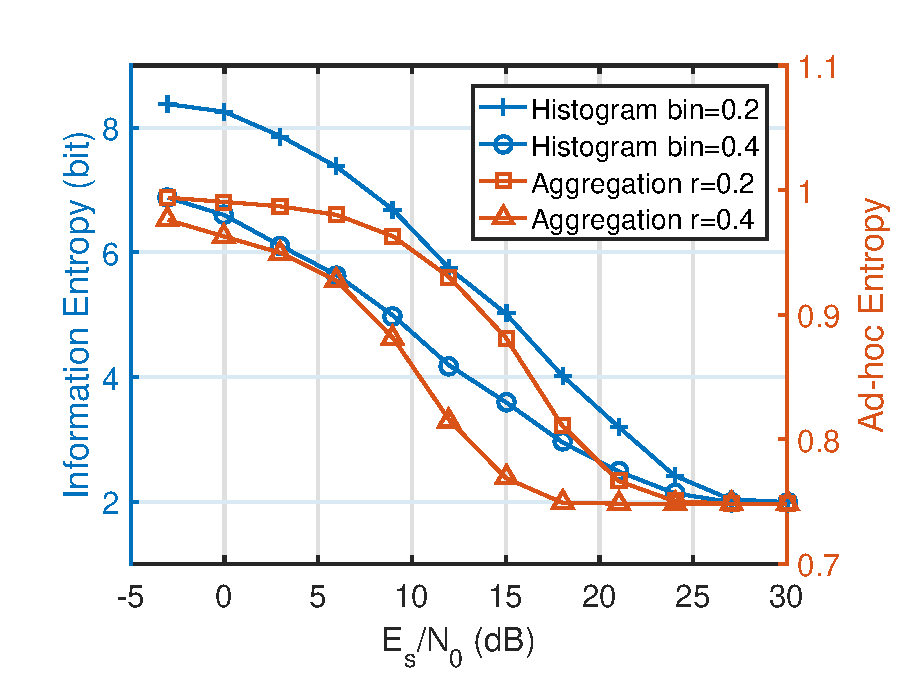
\includegraphics[width=3 in]{pic/adEnt.eps}
\caption{Entropy estimation using two algorithms.}
\label{fig:adEnt} 
\end{figure}
% The additive white Gaussian noise (AWGN) is introduced, where the SNR sweeps from -3 dB to 30 dB.

The 2D histogram based estimation is evaluated for a bin width of 0.2 and 0.4, and the same values are applied to the threshold \(r\) in the ad-hoc entropy estimation.
When the SNR is sufficiently high, the histogram based algorithm reaches the minimum. 
Its value is 2 bits in Fig. \ref{fig:adEnt}, as was predicted by~(\ref{eq:entropy_mid}).

Next let's derive the minimum value of ad-hoc entropy and compare it with the numerical result in Fig. \ref{fig:adEnt}.
Since the symbols are random, there are four groups of symbol points distributed in the constellation diagram, and each group has a number of \(N/4\).
The condition of $d_{ij}>r_{ag}$ can only be satisfied between samples in  groups with different constellation.
For two groups, we have $H_{sp} = (N/4)^2$, so the total $H_{sp} = 6 (N/4)^2$ when four groups are considered.
Thus, the minimum value of the ad-hod entropy is approximated by
\begin{equation}
H_{ad} \approx \frac{ 6 \left(N/4\right)^2}{N^2/2}=0.75.
\label{eq:adEntQPSK}
\end{equation}
which agrees with the results shown in Fig. \ref{fig:adEnt}.


It can be seen that both algorithms are monotonic functions of SNR.
The decreasing entropy reflects the fact that the uncertainty of the system is reduced with the increasing SNR.
This property shows that the proposed algorithm can be used to measure the data randomness.

The choice of the threshold \(r_{ag}\) depends on the energy of signal and noise.
In Fig. \ref{fig:adEnt}, the curve with \(r_{ag}=0.2\) reflects the change of randomness in high SNR region, but saturates for low SNR region, in which case \(r_{ag}=0.4\) is preferred.
This is because the small threshold cannot differentiate the aggregation degree of large scale distributed data samples.
In practice, $r_{ag}$ can be set equal to the RMS value of the noise.

% Similar with ApEn and SampEn algorithms, 
It is best to apply the ad-hoc entropy estimation using a few hundred samples,
because the required distance calculation exhibits quadratic growth with number of data samples. 
The computational pressure can be relieved by either skipping the distance calculation of aggregated samples or using other distance metric (Chebychev etc. \cite{Cha2007ComprehensiveFunctions}).
However, this is not an issue in our application since a reliable synchronization  recovery with less data samples is always preferred, and it is an advantage in tracking the dynamic channel conditions. 
% 跟 histogram 比较性能
% r 选择有什么影响
%%%%%%%%%%%%%%%%%%%%%%%%%%%%%%%%%%%%%%%%%%%%%%%%%%
\section{Symbol Timing and Carrier Frequency Recovery Algorithms}
\label{sec:sync_algo}
In this section, the entropy minimization criterion will be applied to symbol timing and carrier frequency recovery.
The algorithms discussed here work in batch mode, which means the samples are processed block by block. 
It is a direct result of the way entropy is estimated, however, after the initial acquisition, it is not difficult to adapt the algorithms to online mode with a sliding window.
% EM based symbol timing and carrier frequency recovery algorithms



% - configuration: batch search algorithms, timing first and then carrier recovery


\subsection{Symbol Timing Recovery} 
\label{sec:timing}
The symbol timing recovery can be implemented by searching the instant with minimum entropy in the eye diagram.
However, there are several practical issues that need to be addressed.
In the following discussion, we will focus on these topics: the entropy local minimum removal, timing recovery with CFO and the low over sampling rate condition.

The entropy reaches a global minimum in the centre of the eye diagram, but in practice, when the timing instant is close to the symbol transition area, the entropy may go down and creates a local minimum. 
The local minimum is not a big issue if the SNR is high and a global search is applied, but it will deteriorate the performance in low SNR cases or when using gradient based search algorithms.
Since the entropy local minimum occurs when the magnitude is low,  an additional threshold can be introduced to eliminate the data samples with small magnitude in the entropy estimation.
With this idea, the algorithm in Section~\ref{sec:adhoc} is modified to:
\begin{enumerate}

\item Define a threshold \(r_{mg}\) \((r_{mg}>0)\) and build a new samples set where all samples with its magnitude greater than \(r_{mg}\) are included.
The number of samples in the new set is denoted as \(N_{mg}\).
\item Find out all the Euclidean distances \(d_{ij}\) between each sample pair \(x_i\) and \(x_j\) in the new sample set, where \(1\le i<N_{mg}\) and \( i<j \le N_{mg}\). 
\item Define a threshold \(r_{ag}\) \((r_{ag}>0)\) and count the number of \(d_{ij}\) such that $d_{ij}<r$, and denote it as $H_{ag}$.
\item The ad-hoc entropy is given by
\begin{equation}
H_{ad}= 1- \frac{ H_{ag}}{ N(N-1)/2}.
\label{eq:entorpy_ad2}
\end{equation}
\end{enumerate}



A typical case is given here to show how the entropy minimization based symbol timing recovery works.
The received frame consists of 400 QPSK modulated random symbols, 
which are pulse shaped by a RRC filter with a rolloff factor of 0.5 to generate a baseband complex envelop.
An AWGN channel is assumed with $E_s/N_0 = 18~\text{dB}$. 
After the matched filter, the eye diagram of the real component of the signal is plotted in the upper part of Fig. \ref{fig:timing}, and the entropy results estimated by both original and modified algorithms are shown in the lower part,
% as well as its entropy are plotted in , where
where the threshold $r_{ag}=0.25$ and \(r_{mg}=0.3\).
% The ad-hoc entropy estimation algorithm discussed in Section \ref{sec:adhoc} is used to evaluate the timing phase entropy of the eye diagram, where the threshold $r=0.25$.
% The timing phase entropy as a function of normalized timing offset is plotted as a solid red line in the lower part of Fig. \ref{fig:timing}, such that the two figures can be viewed under the same x-axis.

\begin{figure}[htbp]
\centering
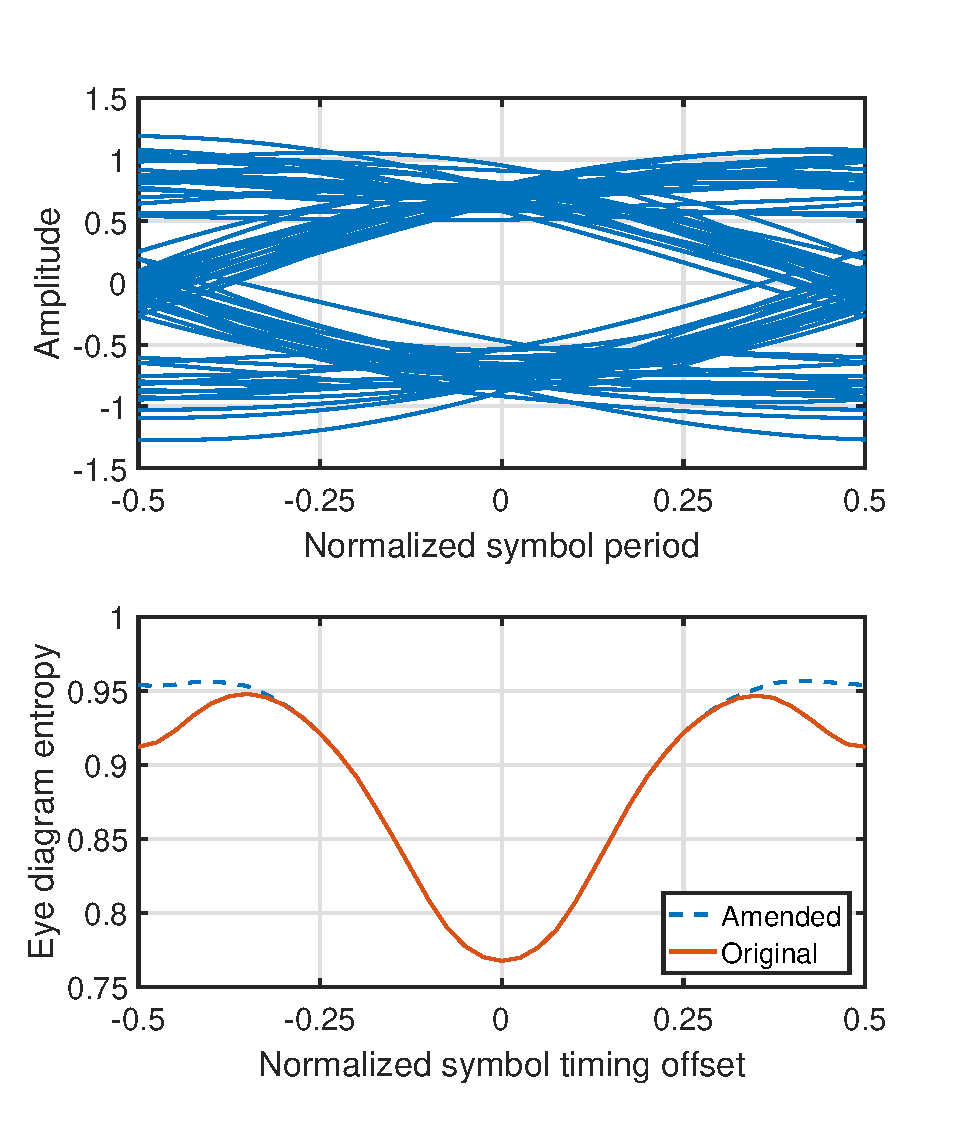
\includegraphics[width=3 in]{pic/timing.eps}
\caption{An typical eye diagram (upper) and the corresponding eye diagram entropy (lower).}
\label{fig:timing} 
\end{figure}

% \subsubsection{Entropy Local Minimum Removal}
From Fig.~\ref{fig:timing}, the entropy reaches a global minimum in the centre of the eye diagram, and its value is close to 0.75 as predicted by~(\ref{eq:adEntQPSK}).
With the increase of timing offset, the entropy increases, indicating  more randomness introduced by the ISI.
When the timing offset is beyond $\pm 0.35$, the  entropy from the original algorithm goes down and creates a local minimum in the symbol transition area. 
% This is because the randomness reduces when the timing phase is close to the symbol transition area.
This phenomenon is also illustrated in the eye diagram, where the samples aggregate into three visible groups (with the amplitudes of \(\pm 1\) and 0).
% The local minimum is not a big issue if the SNR is high and a global search is applied, but it will deteriorate the performance in low SNR cases or when using gradient based search algorithms.

% The ad-hoc entropy estimated by the modified algorithm is also plotted in the lower part of Fig. \ref{fig:timing} where the \(r_{ag}=0.25\).
The entropy estimated by the modified algorithm coincides with the entropy of the original algorithm in most of the timing offsets, but the local minimum near 0.5 becomes flat.
As such, with the modified algorithm, the local entropy minimum due to the symbol transitions is removed and the timing phase recovery can be achieve with higher accuracy.

% \subsubsection{Timing Recovery with Carrier Frequency Offset}
In Fig.~\ref{fig:sysconf}, the timing recovery block is placed before carrier recovery, so the input signal of timing recovery may contain uncompensated CFO.
We shall evaluate the viability of the proposed algorithm in such conditions. 
Theoretically, the previous analysis of timing phase entropy still holds, but the CFO does introduce extra entropy in the estimation.
To understand how the carrier offset affects the timing phase entropy, another simulation is conducted with the same parameters as in the early part of this section.
The only difference is that a CFO at 1\% of symbol rate is considered.
The eye diagram and the corresponding entropy is depicted in Fig. \ref{fig:timing_freq}.
      
\begin{figure}[ht]
\centering
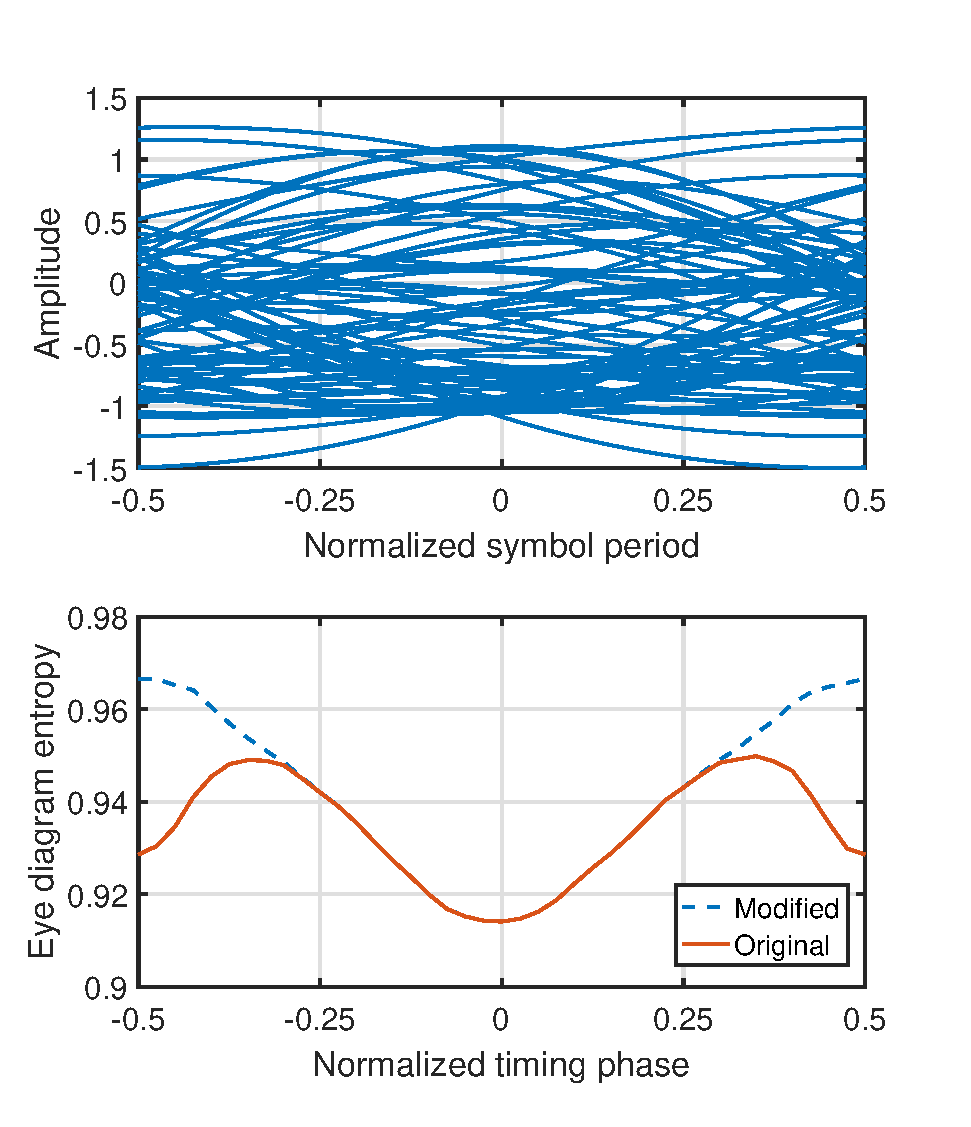
\includegraphics[width=3 in]{pic/timing_freq.eps}
\caption{An eye diagram with carrier frequency offset (upper) and the corresponding eye diagram entropy (lower).}
\label{fig:timing_freq} 
\end{figure}

The eye diagram in the upper part is messy and completely closed. 
There is no way to tell the centre of the eye or optimum timing instant by looking at the eye diagram.
However, the entropy plot tells a different story.
Both the original and the modified algorithms have the same global minimum at 0 timing offset, which means the timing phase entropy based algorithm is immune to the CFO,
but with the price that the entropy value at the minimum is higher than that without frequency offset, i.e., a smaller dynamic range.

Another thing particularly interesting is in the entropy results at symbol transition area.
Using the original algorithm, the local minimum is more noticeable and may lead to a false timing instant.
However, the modified algorithm shows superior performance:
the curve is not flat anymore but continue growing with the same gradient as a function of timing offset.
This feature shows a good adaptation of the modified algorithm, and proves that the `symbol timing before carrier recovery' configuration is feasible.

% \subsubsection{A Feedforward Timing Phase Estimator}
% \label{sec:timing_ff}
A global search for timing phase with minimum eye diagram entropy is not a elegant solution, especially when the high over sampling rate is not available.
The widely used feedforward symbol timing method, the O\&M algorithm uses as low as 4 samples per symbol to estimate the timing phase.

The idea behind the O\&M algorithm is to apply discrete Fourier Transform (DFT) to the squared signal,
and the timing phase is extracted from the angle of the resulting spectrum line at the symbol rate.
The same approach can be applied to EM based algorithm.
To be specific, we can replace the squared signal term in O\&M algorithm with the eye diagram entropy,
such that the the timing phase is given by

\begin{equation}
\tau  = \frac{T}{{2\pi }}\arg \left\{ {\sum\limits_{i = 0}^{N_{sps}-1} {H(k){e^{ - j2\pi i/N_{sps}}}} } \right\},
\label{eq:ff_alg}
\end{equation}
where \(T\) is the symbol period and \(N_{sps}\) is the number of samples per symbol, which should be at least 4 as well.
The operation \(\arg( \cdot )\) returns the phase angles, in radians.
Eye diagram entropy at timing instant \(i\) is denoted as \(H(k)\).
Note that (\ref{eq:ff_alg}) assumes that the entropy curve is symmetric to the centre of the eyediagram,
but it may not stand with high noise level or multipath channels.
It will be further discussed in Section \ref{sec:performance}.

\subsection{Carrier Frequency Recovery}
This section will focus on the EM based carrier frequency recovery algorithm.
Like the symbol timing recovery discussed above, the proposed algorithm does not require the knowledge of data symbols.
The general idea is to multiply the signal by a local carrier with the trial CFO and calculate the corresponding constellation entropy.
Then sweep the trial CFO in a certain range and find the frequency with minimum entropy value.
We will study the characteristic of the entropy curve first and then use a block average method to cope with sharp trough problem.

In the previous discussion, we know that the constellation entropy is almost constant when the CFO is greater than a frequency limit.
Within this frequency limit, the curve has a V-shape trough and the entropy global minimum is located in the middle of the trough.
For a given modulation index, the width of the trough is decided by the CFO \(\Delta f_c\), the symbol rate $f_{sym}$ and the number of data samples $N$ in the window.
For example, the \(M\)-PSK modulated signal has a minimum constellation phase difference \(2\pi/M\).
The accumulated phase shift due to CFO is given by \(2\pi \Delta f_c N / f_{sym}\).
The constellation entropy increases with the CFO until the accumulated phase shift is greater than the minimum constellation phase difference. 
Therefore, trough range is given by
\begin{equation}
\frac{{\left| {\Delta {f_c}} \right|}}{{{f_{sym}}}} < \frac{1}{{MN}}.
\label{eq:freq_limit}
\end{equation}
Beyond that range, the entropy curve is going to be flat.


In (\ref{eq:freq_limit}), if \(N\) is equal to a few hundred, the CFO that can fall into the entropy trough is on the order of 0.1\% of the symbol rate, which is much smaller than the CFO range we want to cover.
The resulting entropy curve as a function of trial CFO is basically flat with a sharp trough, 
so the linear search will require a very small step to achieve high frequency resolution, while a gradient descent algorithm cannot converge due to lack of gradient.
As a consequence, an efficient search algorithm cannot be applied. 

In order to cover a large estimation range without intensive computation, an algorithm that can expand the width of the trough is in demand.
To obtain a wide entropy trough, one possible way is to use less data samples (reduce \(N\)), but that will lead to inaccurate PDF and entropy estimation.
Similar to~\cite{YuanlingHuang2007}, a block average algorithm can be adopted.
\begin{enumerate}
\item The \(N\) data samples are segmented into small blocks, and each of these block has \(L\) samples. There can be overlaps for the blocks to improve the accuracy.
\item Estimate the entropy curve for each block.
\item Average the entropy results from all the blocks.
\end{enumerate}
If the CFO is constant for all the data samples, each block is suppose to have the same entropy curve with random fluctuation.
By averaging the entropy curve from small blocks, a wide and smooth entropy trough is achieved.


With the same settings as in section \ref{sec:timing}, the numerical simulation of the constellation entropy (blue dashed line) is plotted as a function of the CFO.
A perfect symbol timing is assumed, and the CFO is swept within 1\% of the symbol rate.

% The frequency offset under recovery should be smaller than the symbol rate \cite{mengali1997synchronization}.
% To be specific, for \(M\)-PSK modulation schemes, if there are \(N\) samples with sampling interval of \(T_s\), the upper boundary of the frequency offset \(\Delta \omega_c\) is given by
% \begin{equation}
% \Delta \omega_c <\frac{2 \pi}{M N T_s}  
% \label{eq:f_lim}
% \end{equation}
% Regarding the case of QAM signals, the \(2 \pi/M\) in (\ref{eq:f_lim}) should be replaced by the minimum phase difference between their constellation points.

% \subsubsection{}

\begin{figure}[ht]
\centering
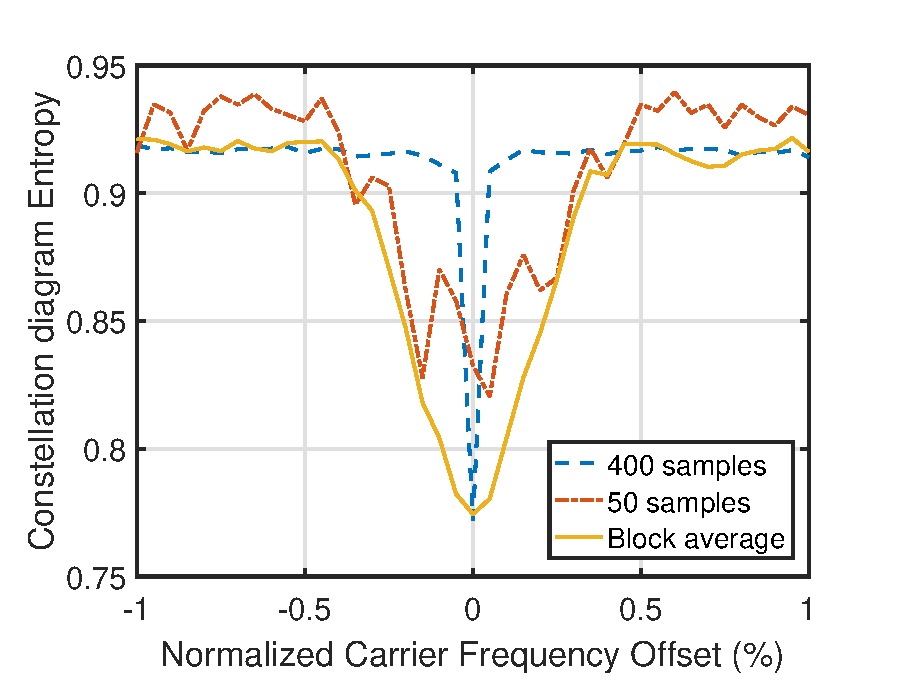
\includegraphics[width=3 in]{pic/freq.eps}
\caption{Constellation diagram entropy for carrier frequency recovery.}
\label{fig:freq_entp} 
\end{figure}   

% \subsubsection{Entropy Curve Expansion}
It is obvious that there is only one global minimum when the CFO is equal to zero and there are no other local minimum as predicted.
In Fig. \ref{fig:freq_entp}, the entropy estimated using 50 samples is also shown.
The trough range is \(\pm 0.5\%\) of symbol rate and it is agree with (\ref{eq:freq_limit}).
Indeed, the trough range is expanded 8 times, but many fluctuations and local minimum show up.
The results from block average algorithm has the same expanded trough as the entropy estimated using 50 samples, but with smooth gradient.

Given the expanded entropy trough, a more efficient two-step linear search is readily to apply.
First, a coarse search through the interested frequency range with half trough wide step size can give us a approximate CFO.
A second search with fine frequency step only sweeps in the frequency range near the coarse estimation result.

Also note that the computation complexity grows quadratically with the number of samples, breaking down into small blocks can significantly reduce the required computation.
In the previous case, if 400 samples is equally divided into 8 blocks without overlap, which is 50 samples per block, it is readily to find it only requires 1/8 of the total computation of Euclidean distance. 


In the above discussion, the CFO in each data batch is estimated and compensated,
but the phase is not considered and there is phase discontinuity between batches.
The initial phase of the data batch should be aligned with the last batch to ensure the phase continuity before the following carrier recovery.
% \subsubsection{Carrier Phase Continuity}
%     - only carrier frequency is recovered, phase different between blocks
%       - keep phase continuity between blocks

% \textbf{to be continued...}
% In high data-rate cases, the synchronization parameters
% (ε, θ, ω) vary slowly in comparison with the symbol interval.
% They can be assumed piecewise constant over a number of
% symbol periods. Synchronization of these quasi-constant parameters
% will be considered here, while tracking of the slowly
% varying parameters can be done in a post-processing unit [3].
%%%%%%%%%%%%%%%%%%%%%%%%%%%%%%%%%%%%%%%%%%%%%%%%%%
\section{Performance Evaluation}
\label{sec:performance}
In this section, the performance of the synchronization algorithms in the previous sections are assessed by numerical simulation.
% The evaluation results are obtained by performing a number of 1000 Monte Carlo trials.
Also, a set of measurement data from an underwater acoustic communication test is synchronized with the EM based algorithm.

\subsection{Numerical Simulation}
% \subsection{Symbol Timing Performance}
\textit{Experiment 1:
Performance of the symbol timing recovery in the presence of AWGN.}
The O\&M algorithm is a batch, feedforward symbol timing estimator.
Since it has the same structure as the proposed feedforward timing recovery algorithm, it is used here to represent the ML based estimator in the performance comparison.

The performance comparison in the presence of AWGN is presented in Fig. \ref{fig:timing_per}.
In this figure, both QPSK and 16-QAM modulation schemes are tested.
A RRC filter with a rolloff factor of 0.25 is used for both pulse shaping and matched filtering.
Complex AWGN is applied to the signal and the symbol energy to noise PSD ratio (\(E_s/N_0\)) ranges from 5 to 40~dB with the step of 5~dB.
For each \(E_s/N_0\) setting, 500 Monte Carlo trials are tested.
In each trial, a block size of 100 samples are evaluated to estimate the timing instant.
After normalization by the symbol period, the variances of the timing instant estimates are plotted in the figure..
It is necessary to compare the results with the theoretical limit.
Following \cite{mengali1997synchronization}, the modified Cram\'er-Rao bound (MCRB) is also plotted as a reference.

\begin{figure}[ht]
\centering
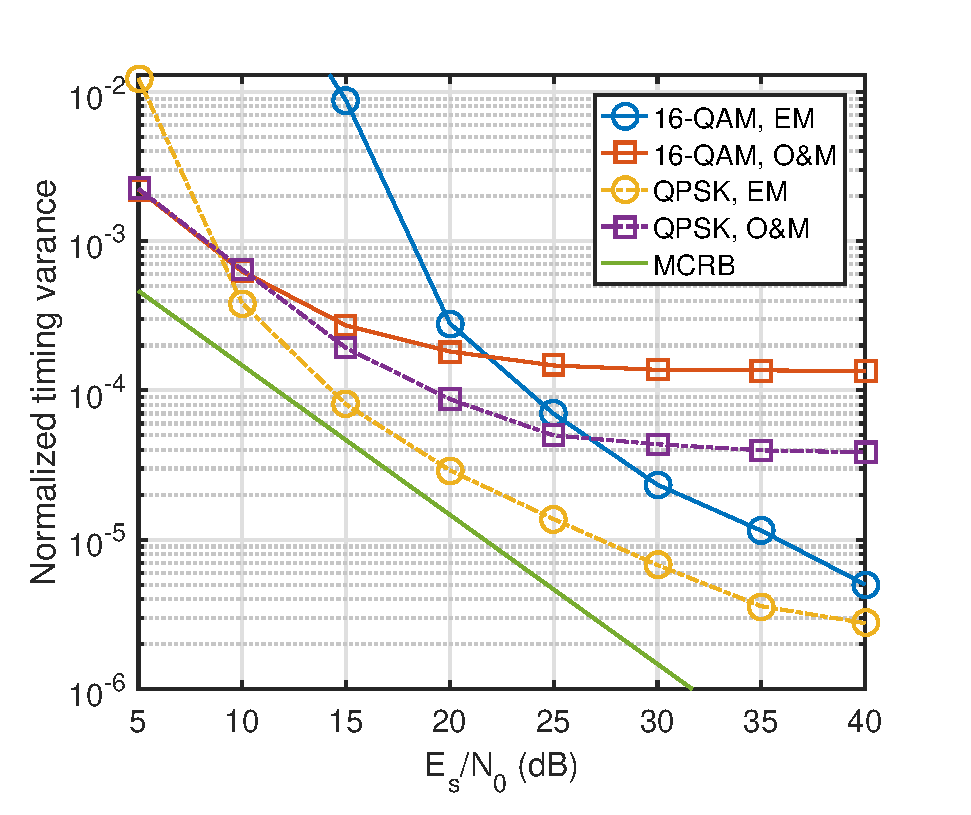
\includegraphics[width=3 in]{pic/per_timing.eps}
\caption{Performance of two symbol timing algorithms with 16-QAM and QPSK modulation schemes.}
\label{fig:timing_per} 
\end{figure}   

Several conclusions can be draw from this figure.
Generally speaking, the EM based symbol timing algorithm has lower variance than the O\&M algorithm for both QPSK and 16-QAM modulation schemes when the  \(E_s/N_0\) is sufficiently high.
% This transition \(E_s/N_0\) is 8~dB for QPSK and 27~dB for 16-QAM
For both algorithms, the low modulation order tends to yield smaller timing variance.
In the high \(E_s/N_0\) region, the performance of O\&M algorithm is limited by the self noise . 
When the \(E_s/N_0\) is greater than 25~dB, the strong self noise due to the small rolloff factor makes O\&M algorithm reaches its lower boundary , while the EM based algorithm doesn't seem to be affected, since  its timing varicance keeps getting smaller with  \(E_s/N_0\).
However, in low \(E_s/N_0\) region, the EM algorithm has inferior performance comparing with ML algorithm.


Note that in the simulation, the rolloff factor is 0.25 ,which means it occupies relative small bandwidth and leading to excessive ISI.
This scenario is in favour of EM based algorithm, since it is looking for the timing instant with minimum ISI.
However, if we have a larger rolloff factor, say 0.75, the O\&M algorithm will have the performance very close to the MCRB \cite{mengali1997synchronization}.
On the other hand, the enlarged signal bandwidth and reduced ISI make the EM based algorithm have inferior performance than the O\&M algorithm.

\textit{Experiment 2:
Performance of the symbol timing recovery in the presence of CFO.}
The EM based symbol timing recovery is insensitive to the CFO, but it is interesting to understand how the performance changes in case of CFO. 
The settings are basically the same as the last simulation, but we will use BPSK and QPSK modulation schemes this time.
The introduced CFO is 1\% of the symbol rate, and the timing variance is plotted in Fig. \ref{fig:timing_frq_per}.

\begin{figure}[ht]
\centering
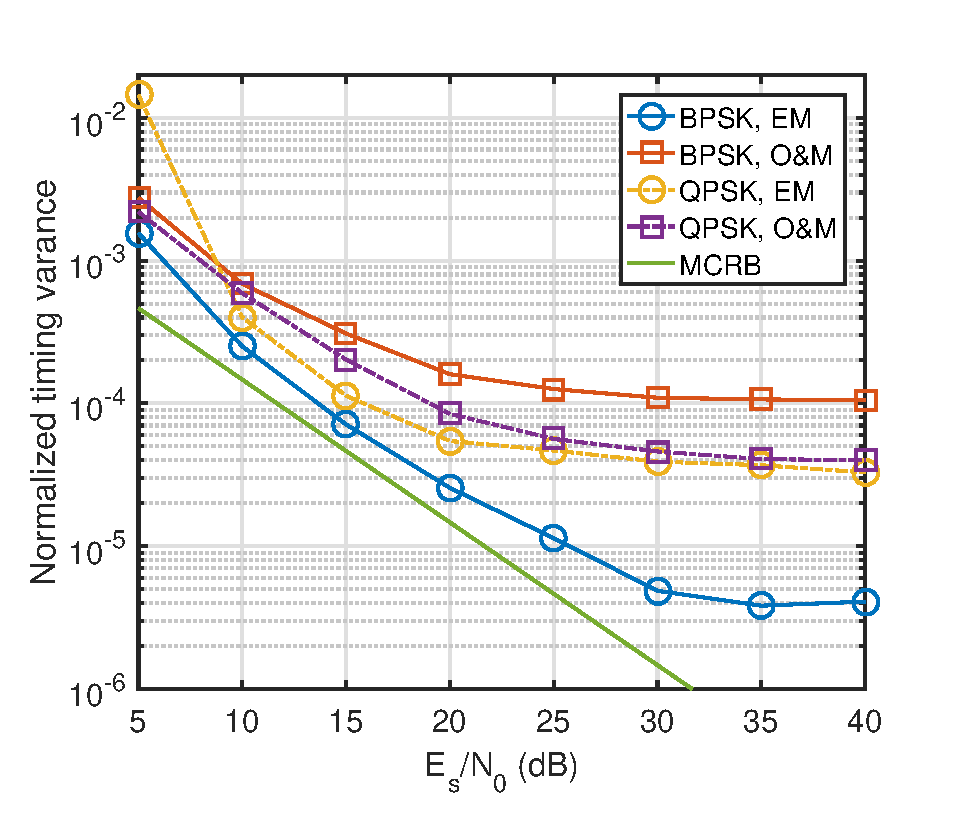
\includegraphics[width=3 in]{pic/per_timing_frq.eps}
\caption{Performance of two symbol timing algorithms in the presence of CFO.}
\label{fig:timing_frq_per} 
\end{figure}  

For the BPSK modulation scheme, EM based algorithm shows good performance that is close to MCRB before \(E_s/N_0\) reaching 30 dB.
It has the highest performance improvement comparing to the O\&M algorithm.
But as to the QPSK modulation scheme, both algorithms have very similar performane curve, and no improvement can be found in this setting.

This is because the EM based algorithm in (\ref{eq:ff_alg}) assumes that the eye diagram entropy curve is symmetrical to the centre of the eye diagram, and this only stands with low modulation order and noise level.
We will show another asymmetrical eye diagram entropy condition in the next simulation. 

\textit{Experiment 3:
EM based symbol timing recovery in multipath channel.}
One of the most important issue a single carrier coherent communication system facing is the multipath channel.
It is interesting to understand how the EM based symbol timing recovery performs in such condition.
Consider a block of BPSK modulated signal which is pulse shaped by the RRC filter with  a rolloff factor of 0.5.
The multipath channel has a impulse response
\begin{equation}
\delta(t)-0.5(t-1.8T).
\end{equation}
and  \(E_s/N_0 = 25 \textrm{ dB}\).  
In the receiver side after the down converter and matched filter, the eyediagram and the corresponding entropy are shown in Fig. \ref{fig:per_timing_isi}. 
\begin{figure}[ht]
\centering
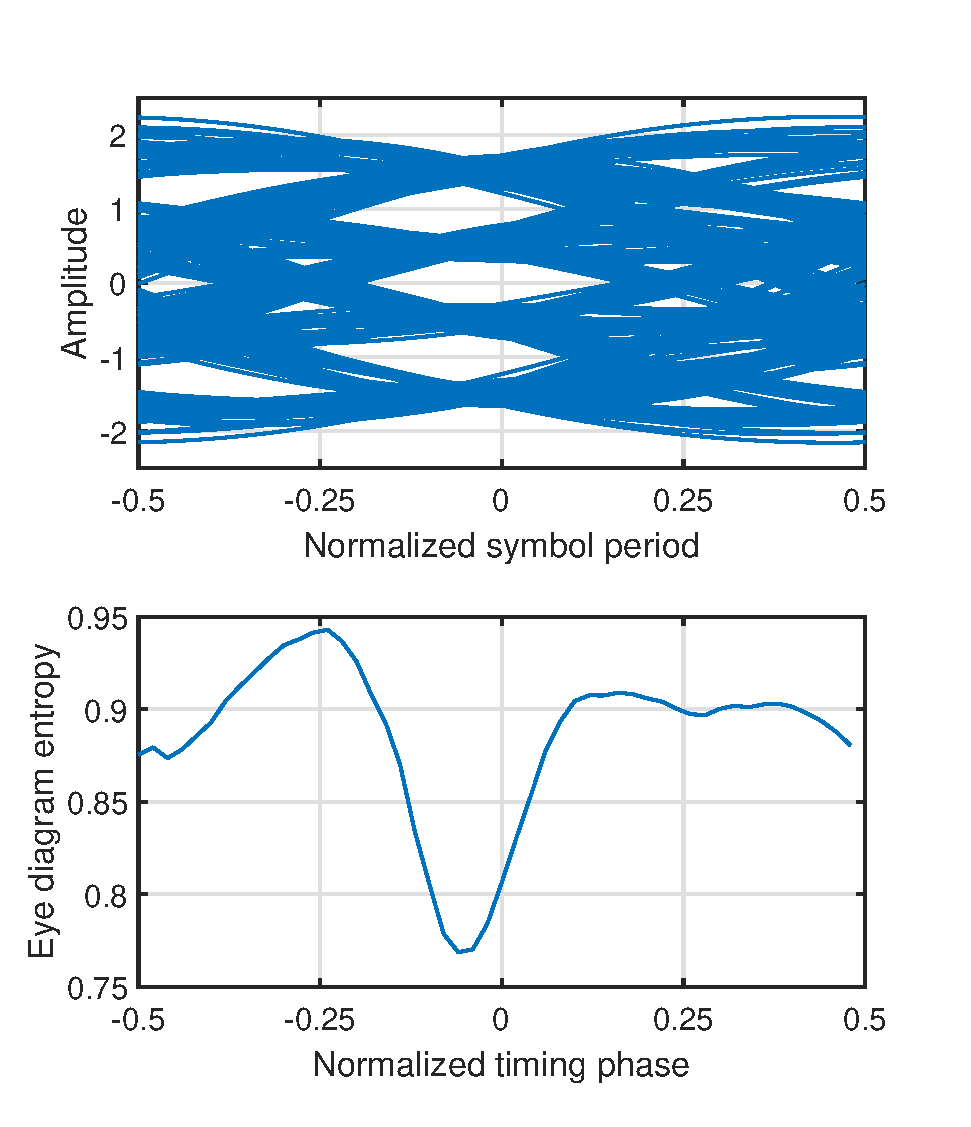
\includegraphics[width=3 in]{pic/per_timing_multi.eps}
\caption{An eye diagram in the presence of ISI (upper) and the corresponding eye diagram entropy (lower).}
\label{fig:per_timing_isi} 
\end{figure} 

In the figure, there is no clear eye opening in the eye diagram, and the entropy curve is asymmetrical to the centre of the eye diagram with both global and local minimum. 
The timing phase with the global minimum is located at \(-0.1\), where the eye diagram has three small eyes at their maximum opening.
The minimum entropy indicates that the least ISI is obtained in this timing instant.
With such the timing instant choice, the equalizer can converge faster and produce stable results.
On the contrary, the timing phase found by ML based timing recovery algorithm is still around 0, 
where the output energy is maximized but with more random ISI.

\textit{Experiment 4:
Performance of carrier frequency recovery in the presence of AWGN.}
In the test of carrier frequency recovery, perfect symbol timing is assumed.
The signal is QPSK modulated with CFO at 1\% of symbol rate.
Two algorithms are employed as the competitor to EM based algorithm to estimate the CFO:
the open loop and the ML algorithm.

The open loop algorithm proposed by \cite{Chuang1991} estimates the CFO  by averaging the differential phase error over the window.
For QPSK modulation, the CFO is given by
\begin{equation}
\Delta f_c = \frac{f_{sym}}{8 \pi } \arg \left\{ {\sum\limits_{i = 1}^{{N} - 1} {{{\big( {x_i x^*_{i-1}} \big)}^4}} } \right\}.
\end{equation}

\begin{figure}[ht]
\centering
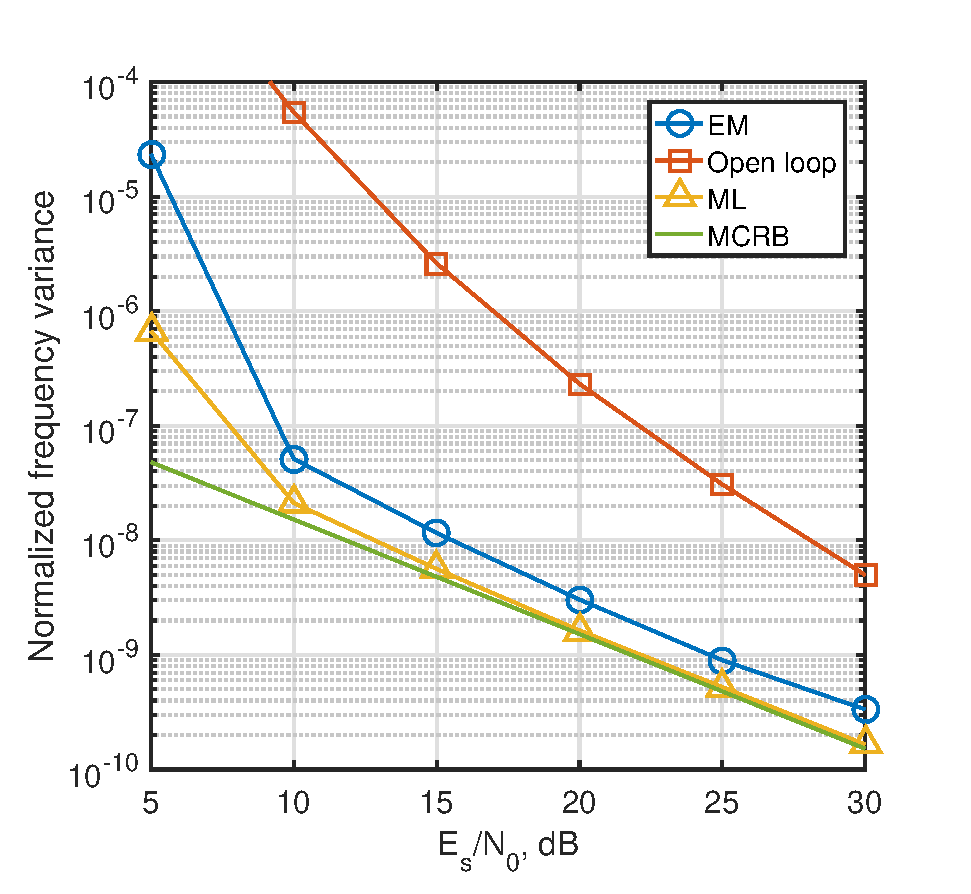
\includegraphics[width=3 in]{pic/per_freq.eps}
\caption{Performance of three carrier frequency recovery algorithms.}
\label{fig:per_freq} 
\end{figure} 

The classic ML algorithm uses the same global search method as the EM based algorithm.
The objective is given by (headache now, not sure if it's right) 
\begin{equation}
\Lambda ({\Delta f_c })=\left| \sum\limits_{k = 1}^N {{{ {{x^4_k}e^{-j8\pi \Delta f_c k T}}}}} \right|. 
\end{equation}
The CFO is estimated by search the trial frequency offset yields the highest energy.
Similarly, the MCRB is also plotted in the figure as the performance reference.

In Fig. \ref{fig:per_freq}, the EM algorithm shows much smaller estimation variance than the open loop algorithm, which proves its excellent carrier frequency recovery performance.
However, the performance of the ML algorithm is mostly the same as the MCRB, making it slightly outperforms the EM based algorithm.

There are several reasons that the EM algorithm may have inferior performance in symbol timing and carrier recovery than the ML based algorithms.
First a few assumptions and approximations are used in the EM algorithms, making it less stable.
The second reason is that the ML algorithms (not its approximations) are theoretically the optimum solution in AWGN channels. 
It is supposed to reach the Cram\'er-Rao bound, therefore, the EM algorithms cannot achieve better performance.
The EM algorithms are more suitable for channels with high order statistics that cannot be neglected.


% test with sea trial measurement data
\subsection{Algorithm Validation with Sea Trial Data }
\label{sec:validation}
In this section, the entropy minimization based synchronization algorithm will be validated with sea trial  measurement data. 
% \subsection{Sea Trial Environment and settings}
The sea trial took place in Northwest Arm near Halifax, NS, Canada on July 6th 2017. The experiment provided an opportunity to evaluate a variety of underwater communications algorithm.
In the test area, the depth is reported to be approximately 10-13 m, and the receiver's deployment location is around 220 m away from the transmitter, and there is certain drift caused by the current.
The sea state is favourable to the test. The acoustic propagation properties can also be observed using the channel impulse response in Fig. \ref{fig:chan_impu}, where there is a strong and stable direct path of arrival and very few multipath interference.
\begin{figure}[htbp]
\centering
\includegraphics[width=2.5in]{pic/channel.png}
\caption{Channel impulse response as a function of time.}
\label{fig:chan_impu} 
\end{figure}

A transmission frame is divided into pilot and data blocks. The pilot block is a wideband, linear frequency modulated chirp signal, which is used for frame synchronization.
The data block is divided into four sections, and each section has a symbol rate of 240, 80, 15 and 5 baud respectively. The data consists of a pseudo-random noise (PN) sequence that has a length of 512 chips, and that is repeated 16 times.
The modulation scheme used is QPSK, and the transmitted waveform is pulse shaped using a raised-cosine filter with a rolloff factor 0.5. The centre frequency is 2.048 kHz. 

% \subsection{Data Processing Results}
% \label{sec:results}
At the receiver, all signals are sampled at 44.1 kHz. The frame is first coarse synchronized with the pilot block so that the data block can be extracted.
Down conversion and a matched filter are applied to the data block to generate the baseband signal.
If the baseband signal is directly down-sampled and demodulated, the bit error rate (BER) is 49\%, which means no information is recovered.

To recover the data, the EM based synchronization algorithm is used before demodulation.
For demonstration purposes, results from 80 baud data are presented here.
In each iteration, 200 symbols are fed into the synchronizer to estimate the timing and carrier frequency offsets. 
The timing and frequency recovery detector outputs are shown in Fig. \ref{fig:per_exp}.

\begin{figure}[ht]
\centering
\includegraphics[width=3 in]{pic/per_exp.eps}
\caption{Synchronization results from EM based algorithms.}
\label{fig:per_exp} 
\end{figure} 

% 先定时还是先频偏? 画出结果
% \begin{figure}[htbp]
% \centering
% \subfigure[Symbol timing offset as a function of time]{
% \label{fig:timing_result}
% \includegraphics[width=3.1in]{timoff.png}}
% % \hspace{0.2in} % 两图间距
% \subfigure[Carrier frequency offset as a function of time]{
% \label{fig:carrier_result}
% \includegraphics[width=3.1in]{freoff.png}}
% \caption{Synchronization results based on entropy minimization criterion.}
% \label{fig:sync_results} %% 总 label
% \end{figure}
There are totally 8192 QPSK symbols for a total duration of 102.4~s.
Both symbol timing and carrier frequency offset are varying with time.
One possible cause is the Doppler effect due to the relative motion between the transmitter and the receiver.

% The synchronized data are depicted in Fig. \ref{fig:scatter}.
After demodulation, the BER is 0.41\%.
As a comparison, with conventional synchronization methods (pilot and PLL based), the BER is 0.49\%.
This result proved that the EM based synchronization algorithm is feasible and can reduce the BER significantly.



%%%%%%%%%%%%%%%%%%%%%%%%%%%%%%%%%%%%%%%%%%%%%%%%%%
\section{Conclusions}
\label{sec:conc}
R\'enyi
\small
\bibliographystyle{IEEEbib}
\bibliography{Mendeley}


\end{document}